\documentclass[12pt]{book}
\usepackage[utf8]{inputenc}
\usepackage{hyperref}
\usepackage{graphicx}

\title{Petit guide d'utilisation de Linux Mint}
\author{Association Eisenia}
\date{2021}

\begin{document}
\maketitle

\newpage
\renewcommand{\contentsname}{Table des matières}
\tableofcontents

\renewcommand{\chaptername}{Chapitre}
\chapter{Introduction}
	\section{Introduction générale}
	\section{Introduction au logiciel libre}

\chapter{Environnement Linux Mint}
\section{Se familiariser avec l'environnement Linux Mint}
	Pour bien commencer avec un nouvel envrironnement, il faut en connaître les bases.
	Savoir bien appréhender les bases de l'environnement, c'est mieux le comprendre et ainsi l'utiliser plus simplement, plus rapidement et se sentir plus à l'aise avec son matériel.\newline
	Dans cette section nous allons voir les éléments basics qui composent l'environnement Linux Mint.
	\subsection{Le bureau}
	Le bureau est le premier élément qui s'affiche sur votre écran une fois votre session ouverte.
	C'est en quelque sorte votre écran d'accueil.
	Il contient des raccourcis vers des fichiers, des dossiers ou encore des applications que vous utilisés fréquement.\newline
	Le but du bureau est de vous faciliter les choses.
	Vous pouvez donc le personnaliser à votre convenance.
	Nous allons voir comment nous pouvons changer le fond d'écran du bureau et comment ajouter et supprimer des éléments sur le bureau.
		\subsubsection{Changement du fond d'écran du bureau}
			Le fond d'écran du bureau est la première chose que l'on voit lorsque l'oon allume l'ordinateur.
			Il est donc préférable que ce fond d'écran nous soit plaisant.\newline
			Une manière très simple de changer de fond d'écran est :
			\begin{enumerate}
				\item Ouvrir le dossier dans lequel se trouve l'image que vous souhaitez mettre en fond d'écran;
				\item Faire clic droit avec la souris sur l'image;
				\item Sélectionner "\texttt{Définir comme arrière-plan du bureau}".
			\end{enumerate}
			Si vous n'avez pas d'image précise que vous souhaitez mettre en fond d'écran mais que vous souhaitez tout de même le changer, vous pouvez faire ceci :
			\begin{enumerate}
				\item Sur le bureau, faire clic droit;
				\item Sélectionner "\texttt{Modifier l'arrière-plan du bureau}";
				\item Une sélection de fonds d'écran vous est proposé. Cliquez sur le fond d'écran qui vous intéressé et il sera immédiatement défini comme fond d'écran du bureau.
			\end{enumerate}
		\subsection{Ajout / suppression d'éléments sur le bureau}
			Si vous utilisez très fréquement un fichier ou un logiciel et que vous ne voulez pas avoir à le chercher à chaque démarrage de votre machine, vous pouvez le mettre sur le bureau. Une petite icône sera alors ajouter au bureau en tant que "raccourcis" vers cet élément. 
			Ainsi, vous n'aurez qu'à cliquer sur cette icône pour ouvrir vos fichiers, vos dossiers ou vos applications favoris.\newline
			Pour mettre un nouvel élément sur votre bureau :
			\begin{enumerate}
				\item Faire clic droit sur l'élément;
				\item Sélectionner "\texttt{Ajouter au bureau}";
				\item Un raccourci a été ajouté sur votre bureau.
			\end{enumerate}
			Si vous ne souhaitez plus voir un élément sur votre bureau, vous pouvez le supprimer du bureau tout en le gardant sur votre ordinateur.\newline
			Attention ! Ceci fonctionne uniquement avec les raccourcis que vous avez créés. Ne faites pas ceci avec un document que vous avez enregistré sur le bureau.
			Le supprimer le supprimera définitivement de votre ordinateur.
			\begin{enumerate}
				\item Sur le bureau, faire clic droit sur l'élément que vous souhaitez enlever du bureau;
				\item Sélectionner "\texttt{Supprimer}" puis confirmer la suppression.
			\end{enumerate}
	\subsection{La barre des tâches}
		La barre des tâches se situe en bas de l'écran.
		Le bouton tout à gauche permet d'ouvrir le "menu démarrer" (voir section \ref{sec:menudemarrer}). 
	\subsection{Le menu démarrer}\label{sec:menudemarrer}
		Le menu démarrer permet d'accéder à l'ensemble des applications qui sont présentes sur votre ordinateur.
		Comme il est ordonné, il est très simple de s'y retrouver et de l'utiliser.
		Ce menu vous sera indispensable.\newline
		Le menu démarrer se décompose en quatre parties :
		\begin{itemize}
			\item La barre latérale tout à gauche contient lesz outils de bases : le Navigateur Firefox (voir Sections \ref{sec:descfirefox} et \ref{sec:utiliserfirefox}); l'invit de commande (voir Section \ref{sec:utiliserterminal}); ...;
			\item Le menu principal au centre contient toutes les catégories de logiciel;
			\item Le menu de droite contient les éléments contenu dans la catégorie sélectionnée;
			\item La barre de recherche en haut permet de rechercher par mots-clés;
		\end{itemize}
	\subsection{Le gestionnaire de fichiers}
		Le gestionnaire de fichiers vous permet de ranger et de retrouver facilement vos dossiers et fichiers divers.\newline
		Le gestionnaire de fichiers se trouve sur la barre des tâches, c'est l'icône qui est représenté par un petit dossier vert.
	\subsection{Extinction de l'ordinateur}
		Lorsque vous avez terminer votre utilisation, il faut éteindre l'ordinateur; L'éteindre après chaque utilisation est important. Cela permet notamment de réduire la chaleur des composants, de résoudre certains bugs liés à une trop longue utilisation, etc.\newline
		Pour cela, ouvrez le menu démarrer et cliquez sur l'icône rouge en bas à gauche de la barre latérale.
		Une boîte de dialogue s'ouvre et vous propose plusieurs options.
		Cliquez sur celle toute à droite "Eteindre".
		Vorte ordinateur affiche le logo de Linux Mint puis s'éteint.
\section{utilisation d'un périphérique amovible}
\section{Paramètrage du compte}
	Dans cette section, nous allons voir comment nous pouvons personnalier l'ordinateur.
	Changer le nom d'utilisateur, le mot de passe, l'avatar... peut être bien utile et plus agréable.\newline
	\subsection{Modifier le nom de l'utilisateur}
	\subsection{Modifier le mot de passe}
	\subsection{Modifier l'avatar}

\chapter{Logiciels}
Dans ce chapitre, nous allons aborder quelques logiciels libres de base pour bien démarrer avec son ordinateur.
Nous présenterons tout d'abord le pack LibreOffice permettant d'éditer une multitude de documents différents.
Puis nous présentenrons le navigateur web Firefox de Mozila.
Enfin, nous présenterons le lecteur multimédia VLC.
La liste de logiciels libres que nous vous proposons ici est non-exhaustive.
Il existe beaucoup d'autres logiciels très pratique selon vos besoins.\
C'est pour quoi, nous expliquons dans la dernière section de ce chapitre comment installer de nouveaux logiciels sur votre ordinateurs.
\section{Les logiciels indispensables pour bien démarrer}
	\subsection{Le pack LibreOffice}
		Le pack LibreOffice est indispensable lorsque l'on souhaite rédiger des documents de toute sorte.\newline
		Il est composé de plusieurs lorgiciels.
		\begin{itemize}
			\item LibreOffice writer vous permet de rédiger des documents textes et de les mettre en forme.
			Ces documents sont au format .odt. 
			Il est aussi possible d'imprimer ses documents ou de les exporter au format .pdf via LibreOffice Writer.
			\item LibreOffice Calc vous permet de créer et d'utiliser des classeurs.
			Ces documents sont au format .ods. 
			Ils sont très utilisés pour faire des feuilles de calculs, enregistrer des données, etc.
			\item LibreOffice Impress vous permet de créer des diaporamas. 
			Ces documents sont au format .odp.
			LibreOffice Impress vous sera très utile pour préparer des supports visuels, des diaporamas pour des exposés, des réunions, etc.
			Il vous sera possible d'exporter votre document au format .pdf.
			\item LibreOffice Draw vous permet de faire toute sorte de dessins.
			Ces documents sont au format .odg.
			Très pratique pour faire un petit dessin rapide, un schéma plus complexe ou bien encore un support visuel.
			\item LibreOffice Math vous permet de rédiger des formules mathématiques.
			Ces documents sont au format .odf;
			Cet outil vous permet de prnedre en notes des formules mathématiquesdiverses, d'utiliser des opérateurs (unitaires, binaires, logiques...), des relations, de rédiger des matrices, d'utiliser des symboles, etc.
			\item LibreOffice Base vous permet de créer et de gérer une base de données relationnelles.
			Il est possible de créer une nouvelle base ou bien de se connecter à une base (JDBC par exemple). 
		\end{itemize}
	\subsection{Mozila Firefox}\label{sec:descfirefox}
		Le navigateur Mozila Firefox va vous permettre d'afficher des pages web.\newline
		Ce navigateur très connu et utilisé vous offre beacoup de paramètres d'affichage, de langue mais aussi de sécurité.\par
		Mozila Firefox est un navigateur libre.
		C'est-à-dire qu'il n'appartient pas à une entreprise dont le but est de faire de l'argent avec ce logiciel.
		Pour un navigateur web, cela garanti notamment une certaine sécurité sur nos données personnelles.
		En effet, Firefox n'a aucun intérêt à revendre les données de ces utilisateurs, donc il en collecte que très peu.\par
		Ce navigateur permet également de bloquer les traqueurs publicitaires.
		...
	\subsection{VLC}

\section{Installer de nouveaux logiciels}
	\textit{Ici, description de l'outil logithèque.}

\chapter{Internet}
Maintenant que nous nous sommes familiarisés avec cet environnement, il est temps d'aller surfer sur le web.\newline
Dans ce chapitre, nous allons voir dans un premier temps comment nous connecter à internet.
Dans un deuxième temps, nous allons mieux étudier le navigateur Mozila Firefox qui sera notre "porte" pour aller sur internet.
Et dans un troisième temps, nous allons voir comment utiliser le moteur de recherche Lilo qui nous permettra de faires nos premières recherches sur internet.
\section{Se connecter à son réseau}
	Avant toute chose, nous devons être connecter à Internet. C'est-à-dire que nous devons établir un lien entre l'ordinateur et le réseau.
	Pour cela, il y a deux façons de procéder :
	\begin{enumerate}
		\item en se connectant via un un câble reliant l'ordinateur à la box ;
		\item en se connectant via un le WiFi.
	\end{enumerate}
	\subsection{Avec un câble éthernet}
		Avec votre ordinateur, un câble RJ45 (éthernet) vous a été fourni.
		L'embout ressemble à ceci :
		\begin{figure}[h]
			\centering
			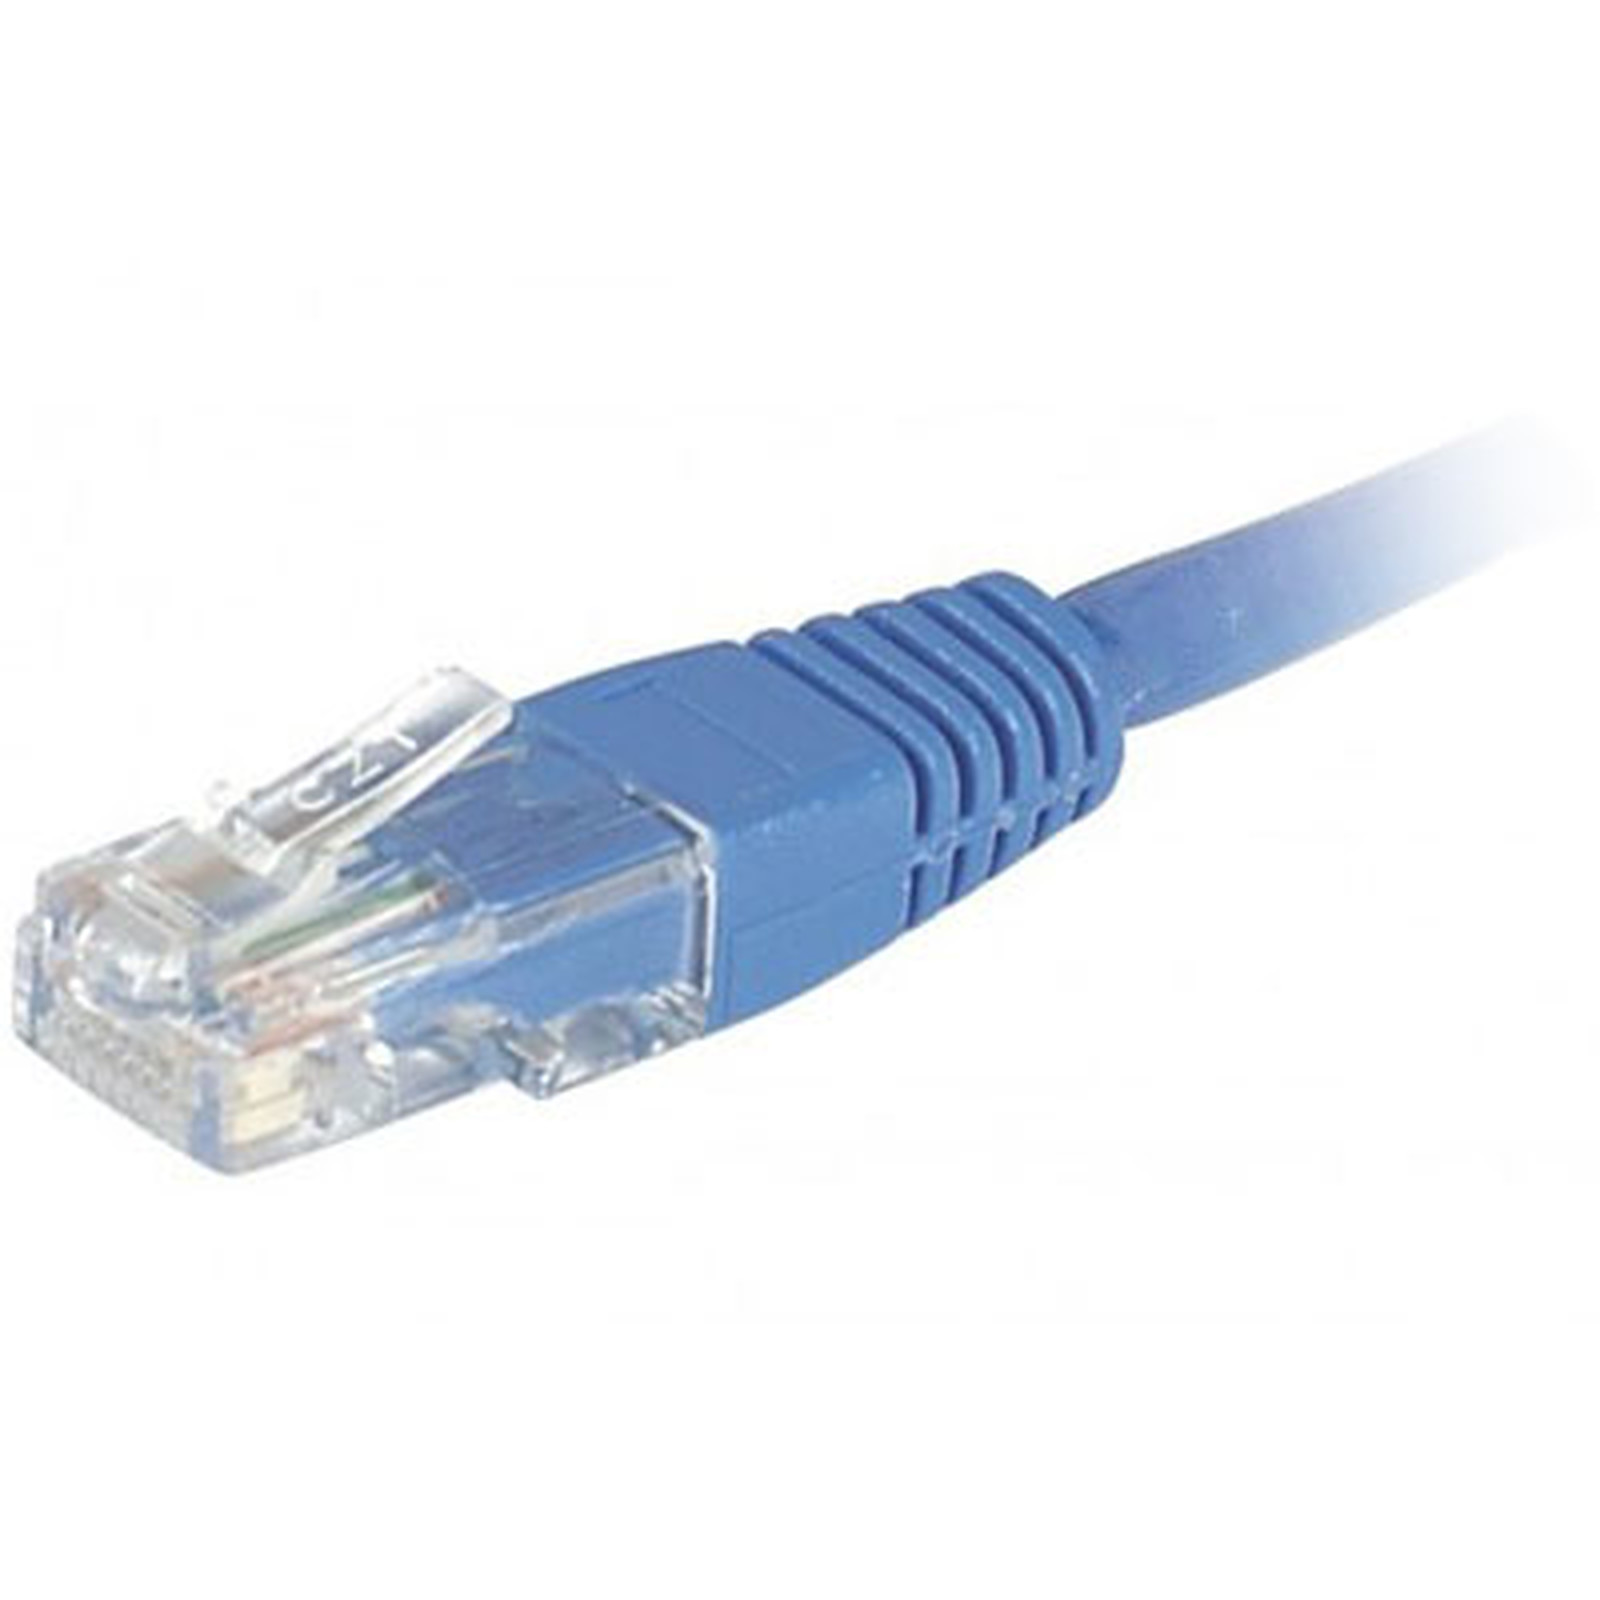
\includegraphics[scale=0.05]{include/rj45.jpg}
			\label{fig:rj45}
			\caption{Câble éthernet RJ45}
		\end{figure}\par
		Ce câble se branche d'un côté à votre ordinateur et de l'autre à votre box (ou dans la prise éthernet de votre mur si elle existe).\par
		Une fois branché des deux côtés, l'icône "Internet" à droite sur la barre des tâches doit avoir changé et ressembler à ceci :
%		\begin{figure}
%			\centering
%			\label{fig:iconeconnecte}
%			\caption{Icône Internet "connecté"}
%		\end{figure}
		\newline
		Une notification a pu aussi apparaître tout en haut à droite de votre écran.
		Elle doit ressember à ceci :
%		\begin{figure}
%			\centering
%			\label{fig:notifconnecte}
%			\caption{Notification "ordinateur connecté" à Internet}
%		\end{figure}
		\newline
		Une fois que cette icône est apparue, félicitations, vous êtes connecté à Internet !
	\subsection{Avec le WiFi}
		Avant de commencer.
		Si vous disposez d'un ordinateur portable, votre ordinateur dispose d'un système de connexion au WiFi intégré et vous pouvez directement essayer de vous connecter.
		Si vous disposez d'un ordinateur fixe, vous aurez probablement besoin d'un dispositif de connexion WiFi externe.
		Nous vous conseillons d'utiliser une clé USB WiFi.
		Elles sont très simple d'utilisation.
		Pour certaines, il suffit de les brancher dans l'ordinateur et vous pourrez vous connecter aux réseaux WiFi.\par
		Pour vous connecter, cliquez sur l'icône "Connexion à Internet" à droite sur la barre des tâches.
		Un petit menu s'affiche alors.
		Cliquez sur le réseau WiFi qui vous intéresse.
		Une boîte de dialogue s'ouvre pour vous demander un mot de passe.
		Entrer le mot de passe de votre réseau et cliquez sur "Entrer".
		Si le mot de passe est incorrect, alors la boîte de dialogue vous demandera à nouveau d'entrer le mot de passe.\par
		Si le mot de passe est le bon, la boîte de dialogue disparait et l'icône "Internet" à droite sur la barre des tâches doit avoir changé et ressembler à ceci :
%		\begin{figure}
%			\centering
%			\label{fig:iconeconnecte}
%			\caption{Icône Internet "connecté"}
%		\end{figure}
		\newline
		Une notification a pu aussi apparaître tout en haut à droite de votre écran.
		Elle doit ressember à ceci :
%		\begin{figure}
%			\centering
%			\label{fig:notifconnecte}
%			\caption{Notification "ordinateur connecté" à Internet}
%		\end{figure}
		\newline
		Une fois que cette icône est apparue, félicitations, vous êtes connecté à Internet !
\section{Utiliser le navigateur Mozila Firefox}\label{sec:utiliserfirefox}
	Nous avons vu dans la Section \ref{sec:deffirefox} de nombreuses informations relatives à ce navigateur libre.
	Si ce n'est pas déjà fait, je vous encourage à lire cette section.\par
	Ici, nous allons voir comment utiliser le navigateur Mozila Firefox.\par
	Pour commencer, ouvrez le navigateur web.
	Pour cela, vous pouvez cliquez sur l'icône "Firefox" qui se trouve sur votre barre des tâche à droite de l'îcône du menu démarrer 
		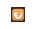
\includegraphics{include/icn_firefox.png}.
	Une nouvelle fenêtre s'ouvre et affiche votre page d'accueil.
\section{Utiliser le moteur de recherche Lilo}
	Lilo est un moteur de recherche. 
	C'est-à-dire qu'il permet, grâce à des mots-clés, de faire des recherches.
	A partir de ces mots-clés, le moteur de recherche va récupérer les pages web les plus pertinentes et les lister.\par
	Lilo est un moteur de rechcerche français. L'avantage de Lilo est triple :
	\begin{itemize}
		\item Lilo n'accepte aucun traqueur.\newline
				Lorsque vous faites une recherche, Lilo ne transmet pas ces données à des comtenus publicitaires ou autres.
		\item Lilo concerve les données personnelles privées.\newline
				Les données personnelles que vous transmettez à Lilo (données de compte, adresse IP, etc.) sont chiffrées et utilisées dans l'unique but de faire fonctionner correctement le moteur de recherche.
		\item Lilo permet de soutenir des projets.\newline
				En faisant vos recherches, vous pouvez choisir d'attribuer des "gouttes d'eau" à un ou plusieurs projets solidaires de votre choix.
				Ces gouttes d'eau sont permettent d'aider à financer ces projets.
	\end{itemize}\par
	Lilo se présente de la manière suivante :
	\begin{enumerate}
		\item La barre de rechercher.
				Tapez les mots-clés pour votre recherche puis appuyer sur la touche \texttt{Entrée}.
		\item Le compteur de gouttes d'eau.
				Visualisez combien de gouttes d'eau vous avez collecté depuis que vous utilisés Lilo.
		\item Le compte Lilo.
				Inscrivez-vous / connectez-vous à votre compte Lilo.
				Ce compte est facultatif.
				Pas besoin d'avoir un compte Lilo pour faire des recherches.
		\item Le menu.
		\begin{enumerate}
			\item \texttt{Accueil} vous permet de revenir à la page de recherche de Lilo.
			\item \texttt{Soutenir un projet} vous permet de sélectionner le (ou les) projet(s) de votre choix en donner vos gouttes d'eau.
			\item \texttt{Proposer un projet} permet à des structures de soumettre leur pojet solidaire à Lilo afin que les internautes puissent leur donner des gouttes d'eau.
			\item \texttt{Vie privée} renvoie vers un descriptif de la gestion des données personnelle par Lilo.
			\item \texttt{FAQ} renvoie vers une page de Questions/Réponses fréquentes.
			\item \texttt{Lilo} renvoie vers une page décrivant le fonctionnement de Lilo.
			\item \texttt{Personnaliser} vous permet d'effectuer des réglages par rapport au moteur de recherche.
			\item \texttt{Mon compte} vous permet de vous connecter ou de vous créer un compte Lilo.
			\item \texttt{Use Lilo in English} vous permet de mettre Lilo en anglais.
			\item Ce compteur affiche le nombre d'euros collectés et reverser par tous les utilisateurs à des projets solidaires.
		\end{enumerate}
		\item Les favoris.
				Accédez plus rapidement à des pages web en les ajoutant à vos favoris LIlo.
				Il s'agit d'une option à ajouter pour qu'elle apparaisse sur la page d'accueil de Lilo.
		\item Le fil d'actualité.
				En descendant sur cette page, vous pouvez consulter les actualités.
				Il s'agit d'une option à ajouter pour qu'elle apparaisse sur la page d'accueil de Lilo.
	\end{enumerate}
	\section{Effectuer sa première recherche sur Internet}
	Pour effectuer une recherche, rien de plus simple ! 
	Rendez-vous sur votre moteur de recherche, nous prendrons comme exemple Lilo.
	Une fois sur la page d'accueil de Lilo, tapez les mots-clés pour votre recherche.
	Par exemple "Pastèque".
	\begin{figure}[h]
		\centering
		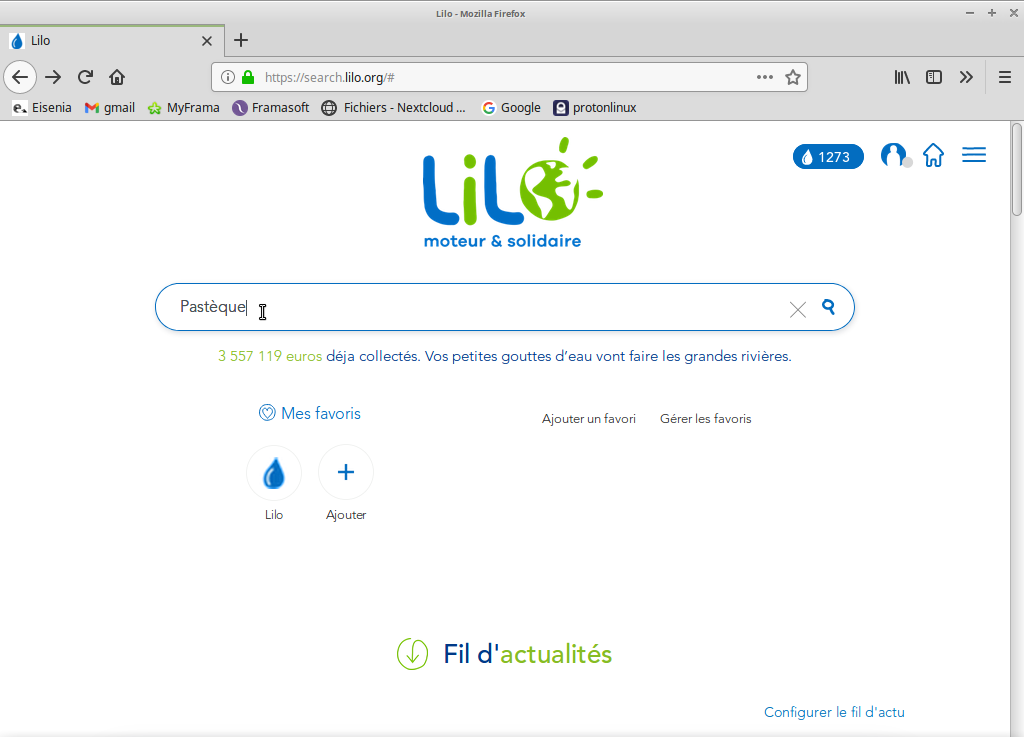
\includegraphics[scale=0.3]{include/pasteque1.png}
		\label{fig:pasteque1}
		\caption{Recherche du mot "Pastèque" dans Lilo}
	\end{figure}
	Appuyer en suite sur la touche \texttt{Entrée} de votre clavier.\par
	Et voilà, le moteur de recherche vous affiche une liste de page web en lien avec le mot clé "Pastèque".
	\begin{figure}[h]
		\centering
		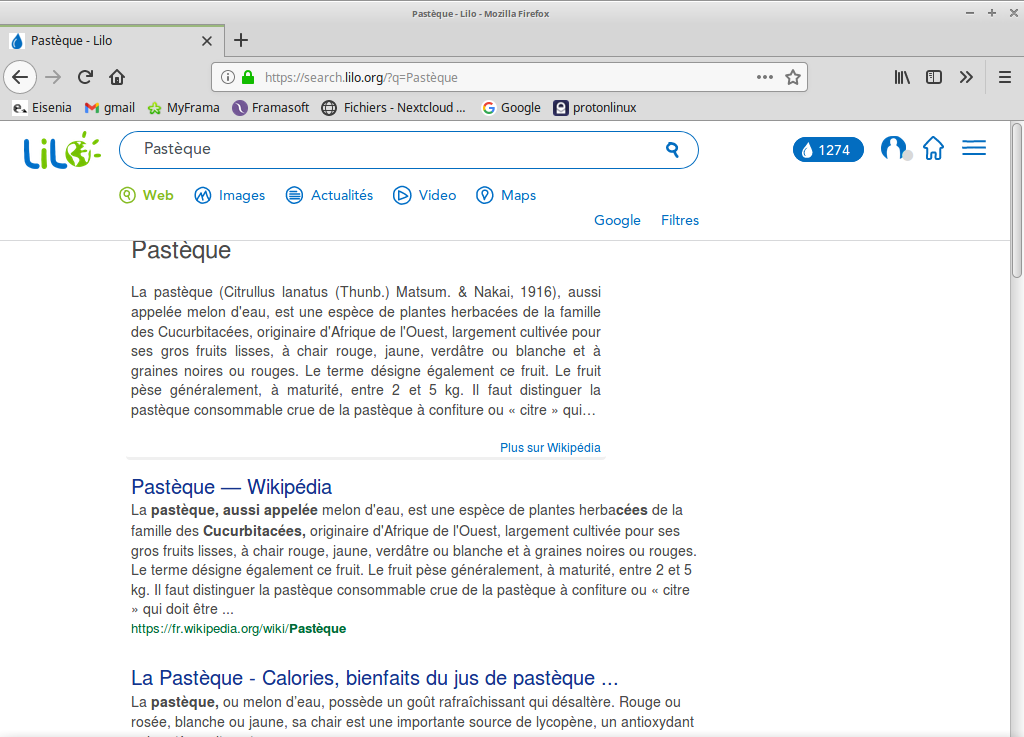
\includegraphics[scale=0.3]{include/pasteque2.png}
		\label{fig:pasteque2}
		\caption{Liste des résultats pour le mot "Pastèque" dans Lilo}
	\end{figure}

\chapter{Mises à jour}\label{sec:maj}
	\section{Pourquoi faire les mises à jour ?}
	\section{Effectuer les mises à jour}

\chapter{Bonnes pratiques}
	\section{Entretien du matériel}
	\section{Sécurité sur internet}

\chapter{Avancé}
\section{Utiliser l'invit de commande}\label{sec:utiliserterminal}
	\subsection{Présentation de l'invit de commande}
	\subsection{Les commandes de bases}


\end{document}